\documentclass[tikz]{standalone}
\usepackage{calc}
\usepackage{tikz}
\usetikzlibrary{matrix,fit,backgrounds,calc,decorations.markings,arrows.meta,shapes.geometric,tikzmark,math}
\usepackage{amsmath}
\usepackage{braket}

\begin{document}
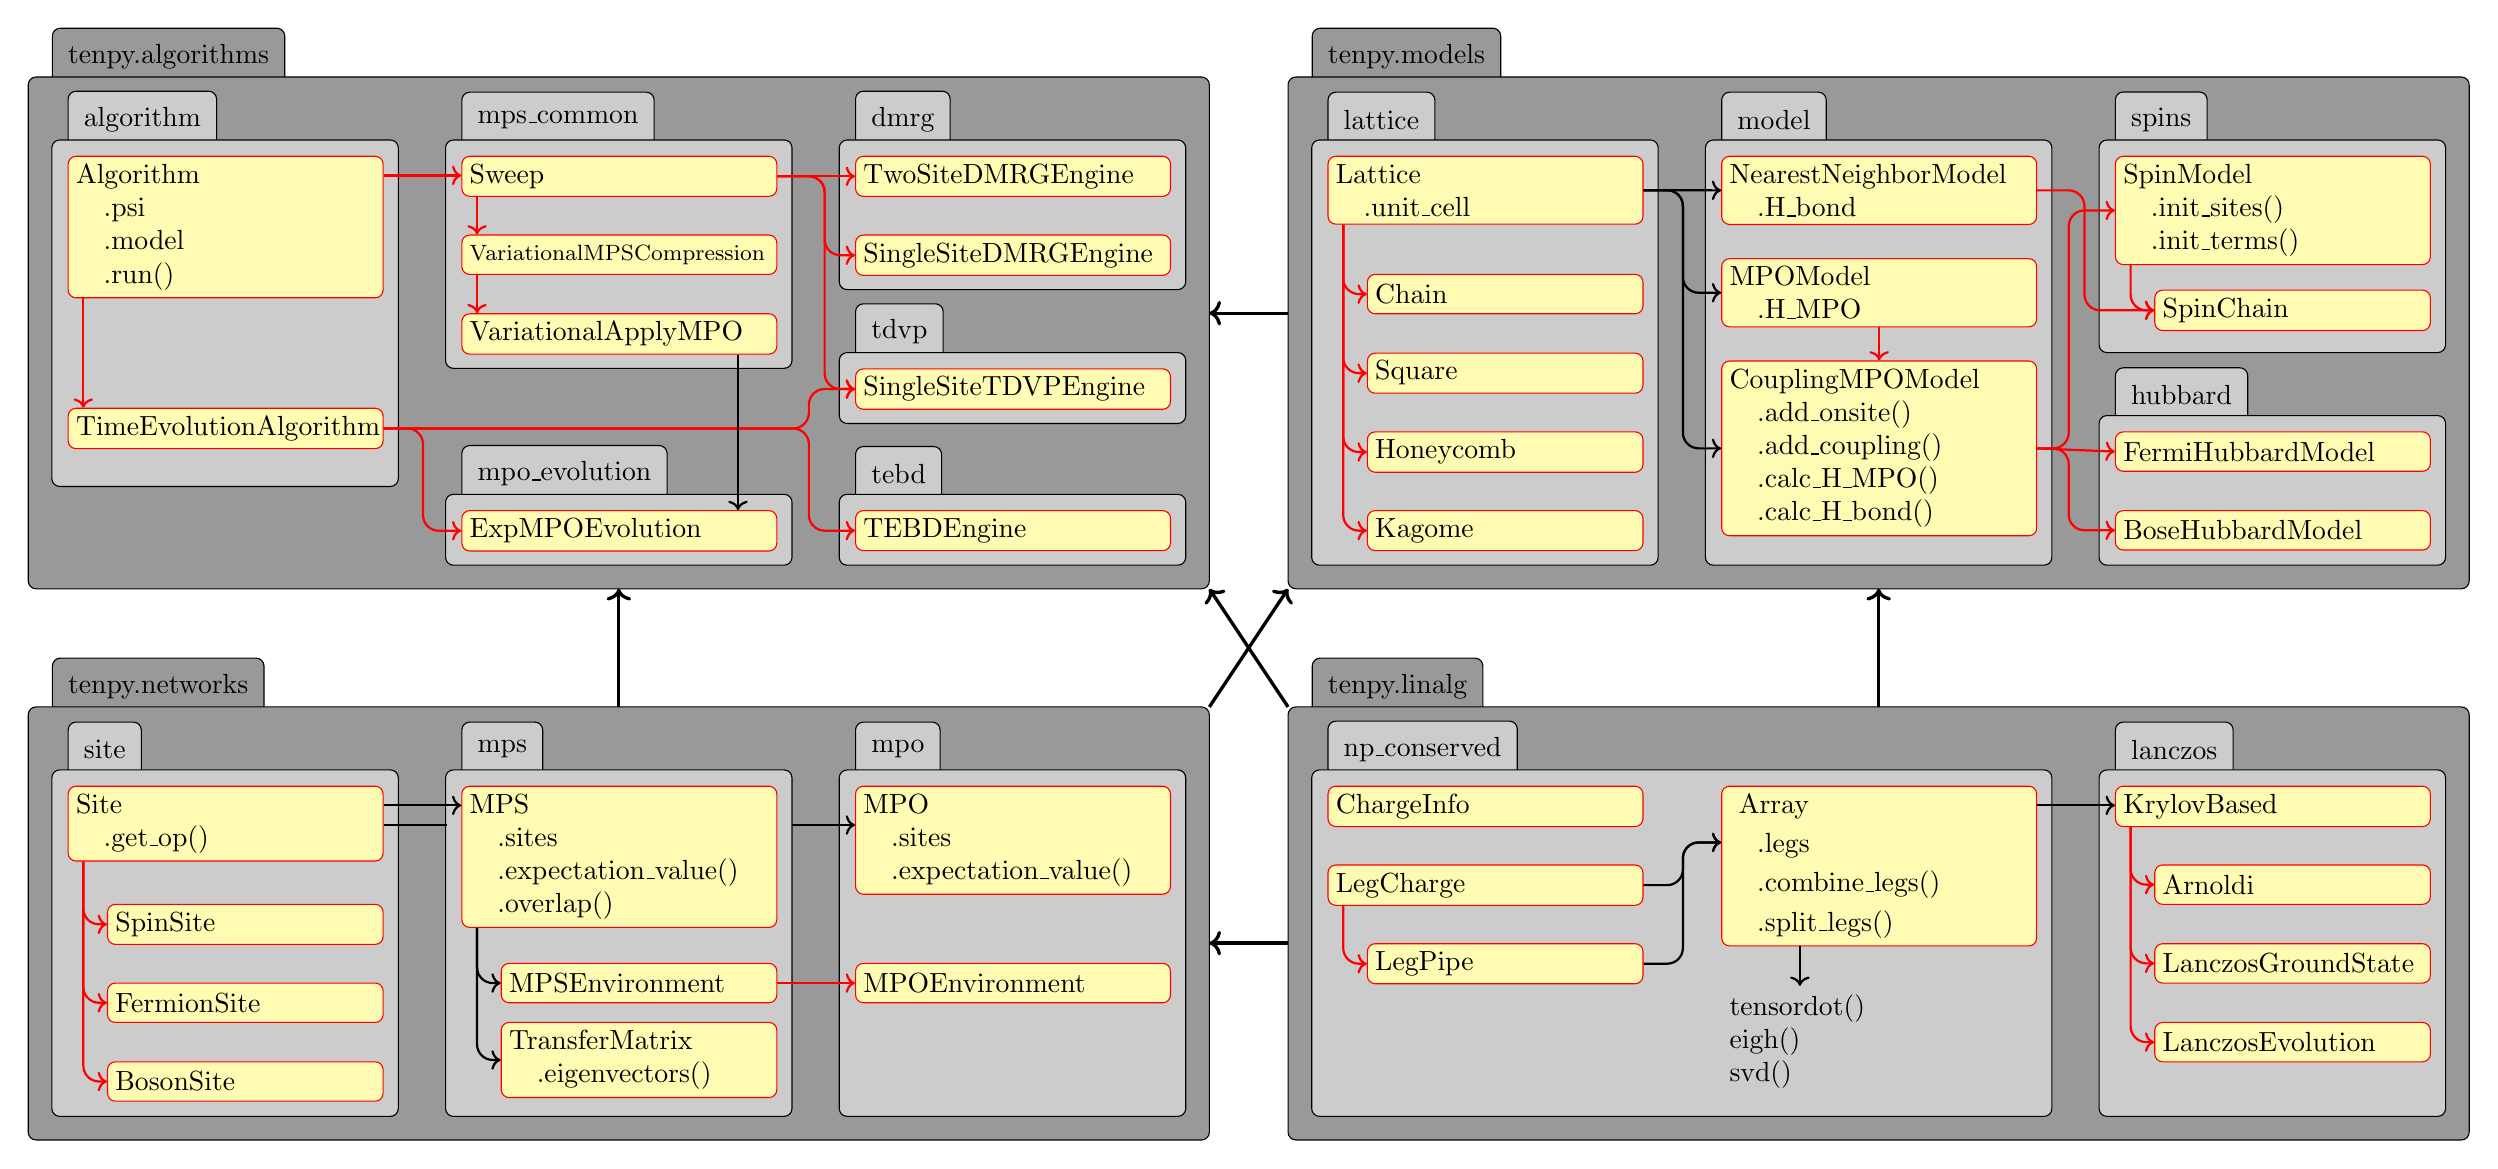
\begin{tikzpicture}[
		remember picture,
		modulecontent/.style={rounded corners=1mm,inner sep=1mm,node font=\texttt,
			minimum height=0.5cm,text width=3.8cm,anchor=north west},
		class/.style={modulecontent,draw=red,fill=yellow!30},
		subclass/.style={class=#1,text width=3.3cm},
		uses/.style={thick,rounded corners=2mm},
		inherit/.style={thick,color=red,rounded corners=2mm},
		%
		package/.style={draw,fill=black!40,rounded corners=1mm,inner sep=2mm},
		subpackage/.style={draw,fill=black!20,rounded corners=1mm,inner sep=2mm},
		pics/package/.style n args={2}{code={
			\node[package,anchor=south west,minimum height=7mm] at (-2mm,9mm) {#1};
			\path[package] (-5mm,10mm)  rectangle ($ #2 + (5mm,-5mm)$) ;
		}},
		pics/subpackage/.style n args={2}{code={
			\node[subpackage,anchor=south west,minimum height=7mm] at (0,1mm) {#1};
			\path[subpackage] (-2mm,2mm)  rectangle ($ #2 + (2mm,-2mm)$) ;
		}}%
	]
	\tikzmath{\colw=5; \classw=4; \subind=0.5;
		%\cb{n} = class begin{n}; \cs{n} = subclass begin; \ce{n} = class end
		\cb1 = 1*\colw - \colw; \cs1 = \cb1 + \subind; \ce1 = \cb1 + \classw ;
		\cb2 = 2*\colw - \colw; \cs2 = \cb2 + \subind; \ce2 = \cb2 + \classw ;
		\cb3 = 3*\colw - \colw; \cs3 = \cb3 + \subind; \ce3 = \cb3 + \classw ;
	}
	%
	\begin{scope}[xshift=0cm,yshift=8cm]
		\draw pic at (\cb1, 0) {package={tenpy.algorithms}{(\ce3,-5)}};
		\draw pic at (\cb1, 0) {subpackage={algorithm}{(\ce1,-4)}};
		\draw pic at (\cb2, 0) {subpackage={mps\_common}{(\ce1,-2.5)}};
		\draw pic at (\cb2, -4.5) {subpackage={mpo\_evolution}{(\ce1,-0.5)}};
		\draw pic at (\cb3, 0) {subpackage={dmrg}{(\ce1,-1.5)}};
		\draw pic at (\cb3, -2.7) {subpackage={tdvp}{(\ce1,-0.5)}};
		\draw pic at (\cb3, -4.5) {subpackage={tebd}{(\ce1,-0.5)}};
		% algorithms
		\node[class]   (Algorithm)   at (\cb1, 0  ) {Algorithm \\ \quad  .psi \\ \quad .model \\ \quad .run() };
		\node[class] (TimeEvolutionAlgorithm)     at (\cb1,-3.2) {TimeEvolutionAlgorithm};
		% mps_common
		\node[class]   (Sweep) at (\cb2 , 0) {Sweep};
		\node[class]   (VariationalMPSCompression) at (\cb2 ,-1) {\footnotesize VariationalMPSCompression};
		\node[class]   (VariationalApplyMPO) at (\cb2 ,-2) {VariationalApplyMPO};
		\node[class]   (ExpMPOEvolution) at (\cb2 , -4.5) {ExpMPOEvolution};
		% dmrg, tdvp, tebd
		\node[class]   (TwoSiteDMRG)     at (\cb3 , 0) {TwoSiteDMRGEngine};
		\node[class]   (SingleSiteDMRG)     at (\cb3 ,-1) {SingleSiteDMRGEngine};
		\node[class]   (SingleSiteTDVP)  at (\cb3 ,-2.7) {SingleSiteTDVPEngine};
		\node[class]   (TEBD)   at (\cb3 ,-4.5) {TEBDEngine};
		\draw[inherit,->] ($ (Algorithm.south west) + (0.2,0) $) -- ($ (TimeEvolutionAlgorithm.north west) + (0.2,0) $) ;
		\draw[inherit,->] ($ (Algorithm.north east) + (0,-0.25) $) -- ($ (Sweep.north west) + (0,-0.25) $) ;
		\foreach \subcls in {SingleSiteDMRG,SingleSiteTDVP}
			\draw[inherit,->] (Sweep.east) -- + (0.6,0) |- (\subcls.west) ;
		\draw[inherit,->] (Sweep.east) --  (TwoSiteDMRG.west) ;
		\draw[inherit,->] ($ (Sweep.south west) + (0.2,0) $) -- ($ (VariationalMPSCompression.north west) + (0.2,0) $) ;
		\draw[inherit,->] ($ (VariationalMPSCompression.south west) + (0.2,0) $) -- ($ (VariationalApplyMPO.north west) + (0.2,0) $) ;
		\foreach \subcls in {SingleSiteTDVP,TEBD}
			\draw[inherit,->] (TimeEvolutionAlgorithm.east) -- + ($ (\colw,0) + (0.4,0) $) |- (\subcls.west) ;
		\draw[inherit,->] (TimeEvolutionAlgorithm.east) -- + (0.5,0) |- (ExpMPOEvolution.west) ;
		\draw[uses,->] ($ (VariationalApplyMPO.south east) + (-0.5,0) $) -- ($ (ExpMPOEvolution.north east) + (-0.5,0) $) ;
	\end{scope}
	%
	\begin{scope}[xshift=16cm,yshift=8cm]
		\draw pic at (\cb1, 0) {package={tenpy.models}{(\ce3,-5)}};
		\draw pic at (\cb1, 0) {subpackage={lattice}{(\ce1,-5)}};
		\draw pic at (\cb2, 0) {subpackage={model}{(\ce1,-5)}};
		\draw pic at (\cb3, 0) {subpackage={spins}{(\ce1,-2.3)}};
		\draw pic at (\cb3, -3.5) {subpackage={hubbard}{(\ce1,-1.5)}};
		% lattice
		\node[class]   (Lattice)   at (\cb1, 0  ) {Lattice \\ \quad  .unit\_cell };
		\node[subclass](Chain)     at (\cs1,-1.5) {Chain};
		\node[subclass](Square)    at (\cs1,-2.5) {Square};
		\node[subclass](Honeycomb) at (\cs1,-3.5) {Honeycomb};
		\node[subclass](Kagome)    at (\cs1,-4.5) {Kagome};
		% models
		\node[class]   (NearestNeighborModel) at (\cb2 , 0)    {NearestNeighborModel \\
			\quad .H\_bond };
		\node[class]   (MPOModel) at (\cb2 ,-1.3)    {MPOModel \\
			\quad .H\_MPO };
		\node[class]   (CouplingMPOModel) at (\cb2 ,-2.6) {CouplingMPOModel \\
			\quad .add\_onsite() \\
			\quad .add\_coupling() \\
			\quad .calc\_H\_MPO() \\
			\quad .calc\_H\_bond() };
		% spins
		\node[class]   (SpinModel)          at (\cb3 , 0) {SpinModel \\ \quad .init\_sites() \\ \quad .init\_terms()};
		\node[subclass](SpinChain)          at (\cs3 ,-1.7) {SpinChain};
		\node[class]   (FermiHubbardModel)  at (\cb3 ,-3.5) {FermiHubbardModel};
		\node[class]   (BoseHubbardModel)   at (\cb3 ,-4.5) {BoseHubbardModel};
		%
		\draw[uses,->] (Lattice.east) -- (NearestNeighborModel.west);
		\foreach \dest in {MPOModel,CouplingMPOModel}
			\draw[uses,->] (Lattice.east) -- +(0.5,0) |- (\dest.west);
		\foreach \subcls in {Chain,Square,Honeycomb,Kagome}
			\draw[inherit,->] ($ (Lattice.south west) + (0.2,0) $) |- (\subcls.west) ;
		\foreach \subcls in {SpinModel,BoseHubbardModel}
			\draw[inherit,->] (CouplingMPOModel.east) -- +(0.4,0) |- (\subcls.west) ;
		\draw[inherit,->] (CouplingMPOModel.east) -- (FermiHubbardModel.west) ;
		\draw[inherit,->] (NearestNeighborModel.east) -- +(0.6,0) |- (SpinChain.west) ;
		\draw[inherit,->] ($ (SpinModel.south west) + (0.2,0) $) |- (SpinChain.west) ;
		\draw[inherit,->] (MPOModel.south) -- (CouplingMPOModel.north) ;
	\end{scope}
	%
	\begin{scope}[xshift=0cm,yshift=0cm]
		\draw pic at (\cb1, 0) {package={tenpy.networks}{(\ce3,-4)}};
		\draw pic at (\cb1, 0) {subpackage={site}{(\ce1,-4)}};
		\draw pic at (\cb2, 0) {subpackage={mps}{(\ce1,-4)}};
		\draw pic at (\cb3, 0) {subpackage={mpo}{(\ce1,-4)}};
		\node[class]   (Site)         at (\cb1 , 0)    {Site \\ \quad  .get\_op() };
		\node[subclass](SpinSite)     at (\cs1, -1.5)   {SpinSite};
		\node[subclass](FermionSite)  at (\cs1, -2.5) {FermionSite};
		\node[subclass](BosonSite)    at (\cs1, -3.5) {BosonSite};
		\node[class]   (MPS)         at (\cb2 , 0)    {MPS \\
			\quad .sites \\
			\quad .expectation\_value() \\
			\quad .overlap() };
		\node[class]   (MPO)         at (\cb3 , 0)    {MPO \\
			\quad .sites \\
			\quad .expectation\_value()};
		\node[subclass]   (MPSEnvironment)         at (\cs2 , -2.25)    {MPSEnvironment };
		\node[subclass]   (TransferMatrix)         at (\cs2,-3)    {TransferMatrix \\ \quad .eigenvectors()};
		\node[class]   (MPOEnvironment)         at (\cb3 , -2.25)    {MPOEnvironment };
		%
		\draw[uses,->] ($ (Site.north east) + (0,-0.25) $) --  ($ (MPS.north west) + (0,-0.25) $);
		\draw[uses] ($ (Site.north east) + (0,-0.5) $) --  +(0.8,0);
		\draw[uses,->] ($ (MPO.north west) + (-0.8,-0.5) $) -- +(0.8,0);
		\foreach \dest in {MPSEnvironment,TransferMatrix}
			\draw[uses,->] ($ (MPS.south west) + (0.2,0) $) |- (\dest.west) ;
		\foreach \subcls in {SpinSite,FermionSite,BosonSite}
			\draw[inherit,->] ($ (Site.south west) + (0.2,0) $) |- (\subcls.west) ;
			\draw[inherit,->] (MPSEnvironment.east) -- (MPOEnvironment.west) ;
	\end{scope}
	%
	\begin{scope}[xshift=16cm,yshift=0cm]
		\draw pic at (\cb1, 0) {package={tenpy.linalg}{(\ce3,-4)}};
		\draw pic at (\cb1, 0) {subpackage={np\_conserved}{(\ce2,-4)}};
		\draw pic at (\cb3, 0) {subpackage={lanczos}{(\classw,-4)}};
		\node[class]   (ChargeInfo) at (\cb1, 0) {ChargeInfo};
		\node[class]   (LegCharge)  at (\cb1, -1) {LegCharge};
		\node[subclass](LegPipe)    at (\cs1, -2) {LegPipe};
		%
		\node[class]   (Array)      at (\cb2, 0) {
			\setlength{\baselineskip}{0.5cm}
			Array \\
			\quad .legs \\
			\quad .combine\_legs() \\
			\quad .split\_legs() \\
		};
		\node[modulecontent] (npc_fct) at ($ (Array.south west) + (0,-0.5) $) {tensordot() \\ eigh() \\ svd()};
		%
		\node[class] (KrylovBased) at (\cb3, 0) {KrylovBased};
		\node[subclass] (Arnoldi) at (\cs3, -1) {Arnoldi};
		\node[subclass] (LanczosGroundState) at (\cs3, -2) {LanczosGroundState};
		\node[subclass] (LanczosEvolution) at (\cs3, -3) {LanczosEvolution};
		%
		\draw[inherit,->] ($ (LegCharge.south west) + (0.2,0) $) |- (LegPipe.west) ;
		\foreach \src in {LegCharge,LegPipe}
			\draw[uses,->] (\src.east) -- +(0.5,0) |- ($ (Array.west) + (0,0.3) $);
		\draw[uses,->] ($ (Array.south west) + (1,0) $) --  ($ (npc_fct.north west) + (1,0) $);
		\draw[uses,->] ($ (Array.north east) + (0,-0.25) $) --  ($ (KrylovBased.north west) + (0,-0.25) $);
		\foreach \subcls in {Arnoldi,LanczosGroundState,LanczosEvolution}
			\draw[inherit,->] ($ (KrylovBased.south west) + (0.2,0) $) |- (\subcls.west) ;
	\end{scope}
	\draw[very thick,->] (15.5, -2) -- (14.5,-2);
	\draw[very thick,->] (15.5, 6) -- (14.5,6);
	\draw[very thick,->] (7, 1) -- (7,2.5);
	\draw[very thick,->] (23, 1) -- (23,2.5);
	\draw[very thick,->] (15.5, 1) -- (14.5,2.5);
	\draw[very thick,->] (14.5, 1) -- (15.5,2.5);
	% % coordinates
	% \draw[very thin, color=blue] (-2.0,-5.0) grid (30.0,15.0);
	% \draw[thick,color=blue,->] (-2.,0) -- (35., 0.) ;
	% \draw[thick,color=blue,->] (0., -5.) -- (0., 15) ;
	% \foreach \i in {-3,...,15}
	% {
	%     \node at (0,\i) {\i{}};
	%     \node at (\i,0) {\i{}};
	% }
\end{tikzpicture}
\end{document}
